\setcounter{figure}{0}
\setcounter{table}{0}
\setcounter{page}{1}
\renewcommand{\thefigure}{Figure~S\arabic{figure}}
\renewcommand{\thetable}{Table~S\arabic{table}}
\renewcommand{\thepage}{S\arabic{page}}
  
%%% TITLE %%%
%\title{\huge \bf Supporting Information:\\ \vspace{0.5cm} \Large Canalization of the evolutionary trajectory of the human influenza virus}
%\maketitle

\section*{Supporting Information}

%%% Figure S1: phenotypes %%%
\vspace*{\fill}
\begin{figure}[H]
	\centering
	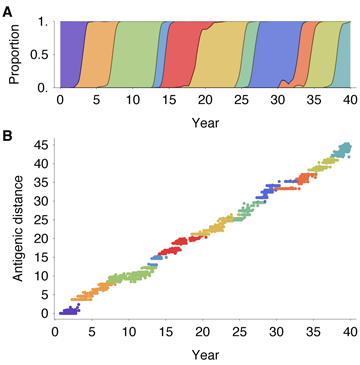
\includegraphics{figures/phenotypes}
	\caption{\textbf{Antigenic evolution over the course of the 40-year simulation}. (A) Proportion of virus population comprised of each antigenic cluster through time.  (B) Antigenic distance from initial phenotype ($x=0$, $y=0$) for each of 5943 virus samples relative to time of virus sampling.  Viruses were sampled at a constant rate proportional to prevalence and coloring was determined from the antigenic map in \ref{evol}D.}
	\label{phenotypes}
\end{figure}
\vspace*{\fill}

\pagebreak

%%% Figure S2: driftvsinc %%%
\vspace*{\fill}
\begin{figure}[H]
	\centering
	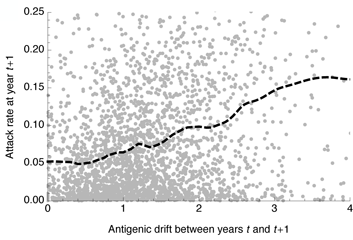
\includegraphics{figures/driftvsinc}
	\caption{\textbf{Correlation between antigenic drift and attack rate}. Antigenic drift is measured as the distance between the centroid of phenotypes of one year and the centroid of phenotypes of the following year.  Measurements were taken across 80 replicate simulations.  Individual pairs of measurements are shown as gray points and a locally-linear regression (LOESS) is shown as a black dashed line.}
	\label{driftvsinc}
\end{figure}
\vspace*{\fill}

\pagebreak

%%% Figure S3: incmaptree_smooth %%%
\vspace*{\fill}
\begin{figure}[H]
	\centering
	\makebox[\textwidth]{
		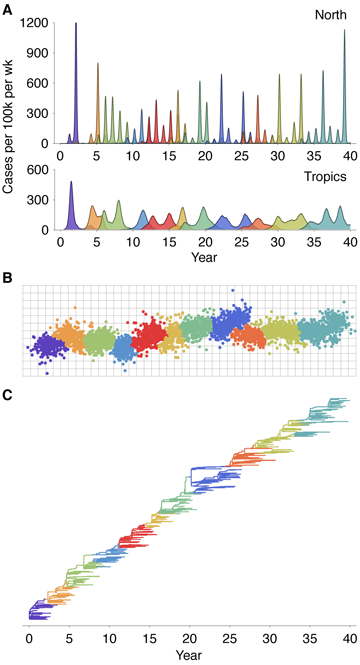
\includegraphics{figures/incmaptree_smooth}
	}
	\caption{\textbf{Simulation results showing epidemiological, antigenic and genealogical dynamics for `smoother' mutation model}. (A) Weekly timeseries of incidence of viral infection in north and tropics regions. (B) Antigenic map depicting phenotypes of viruses sampled over the course of the simulation.  Grid lines show single units of antigenic distance. (C) Genealogical tree depicting the infection history of samples from the virus population.  Cluster assignments were used to color panels (A), (B) and (C) in a consistent fashion.  Alternative mutational parameters are $\mu = 3 \times 10^{-4}$, mean mutation size of 0.6 units and standard deviation of mutation size of 0.2 units.}
	\label{incmaptree_smooth}
\end{figure}
\vspace*{\fill}

\pagebreak

%%% Figure S4: incmaptree_rough %%%
\vspace*{\fill}
\begin{figure}[H]
	\centering
	\makebox[\textwidth]{
		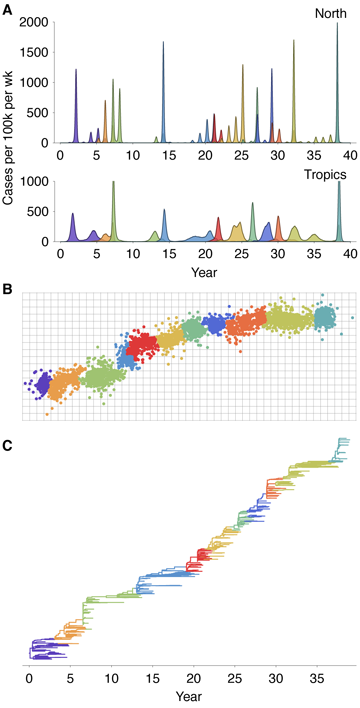
\includegraphics{figures/incmaptree_rough}
	}
	\caption{\textbf{Simulation results showing epidemiological, antigenic and genealogical dynamics for `rougher' mutation model}. (A) Weekly timeseries of incidence of viral infection in north and tropics regions. (B) Antigenic map depicting phenotypes of viruses sampled over the course of the simulation.  Grid lines show single units of antigenic distance. (C) Genealogical tree depicting the infection history of samples from the virus population.  Cluster assignments were used to color panels (A), (B) and (C) in a consistent fashion.  Alternative mutational parameters are $\mu = 5 \times 10^{-5}$, mean mutation size of 0.7 units and standard deviation of mutation size of 0.5 units.}
	\label{incmaptree_rough}
\end{figure}
\vspace*{\fill}

\pagebreak

%%% Figure S5: mutspectrum %%%
\vspace*{\fill}
\begin{figure}[H]
	\centering
	\makebox[\textwidth]{		
		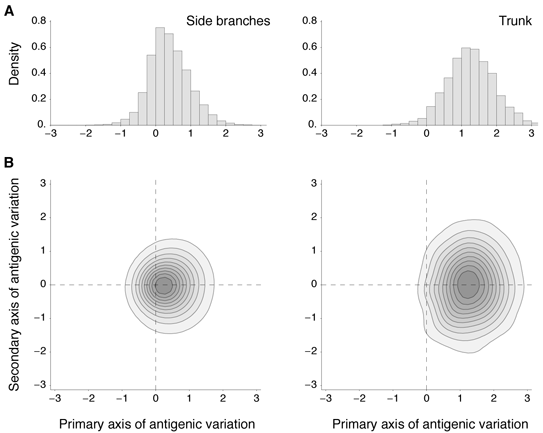
\includegraphics{figures/mutspectrum}
	}
	\caption{\textbf{Mutation spectrum in two-dimensional antigenic space of side branch mutations and trunk mutations}. (A) Histogram of mutation effects along the axis of primary antigenic variation across 80 replicate simulations.  The left panel shows the distribution of effects of side branch mutations and the right panel shows the distribution of effects of trunk mutations. (B) Smoothed two-dimensional histogram of mutation effects along the primary and secondary axes of antigenic variation across 80 replicate simulations.  Histograms were constructed from 21,405 side branch mutations and 1584 trunk mutations.}
	\label{mutspectrum}
\end{figure}
\vspace*{\fill}

\pagebreak

%%% Figure S6: probtrunk %%%
\vspace*{\fill}
\begin{figure}[H]
	\centering
	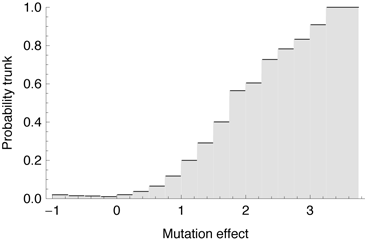
\includegraphics{figures/probtrunk}
	\caption{\textbf{Relationship between a mutation's phenotypic effect and its likelihood of being part of the trunk}. The $x$-axis represents the effect of a mutation along the line of primary antigenic variation, and the $y$-axis represents the probability that the mutation is part of the trunk.  Mutations of large effect are increasingly rare, but when they do occur are increasingly likely to be part of the trunk.}
	\label{probtrunk}
\end{figure}
\vspace*{\fill}

\pagebreak

%%% Figure S7: waittimes %%%
\vspace*{\fill}
\begin{figure}[H]
	\centering
	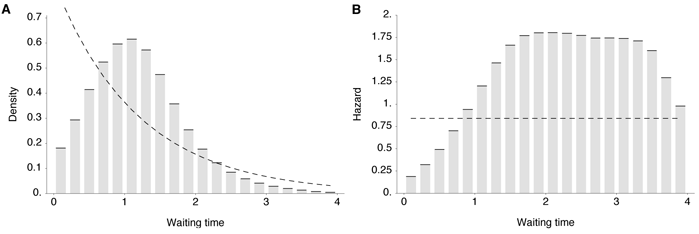
\includegraphics{figures/waittimes}
	\caption{\textbf{Observed vs.\ expected distributions of waiting times between phenotypic mutations along genealogy trunk.} (A) Histogram bins show the observed distribution of waiting times in years across 80 replicate simulations representing 1584 mutations.  The mean of this distribution is 1.76 years.  The dashed line shows the Poisson process expectation of exponentially distributed waiting times.  (B) The density distribution of waiting times is transformed into a hazard function, representing the rate of trunk mutation after a specific waiting time.  The dashed line shows the memoryless hazard function of the Poisson process expectation.}
	\label{waittimes}
\end{figure}
\vspace*{\fill}

\pagebreak

%%% Figure S8: h1n1_mut %%%
\vspace*{\fill}
\begin{figure}[H]
	\centering
	\makebox[\textwidth]{
		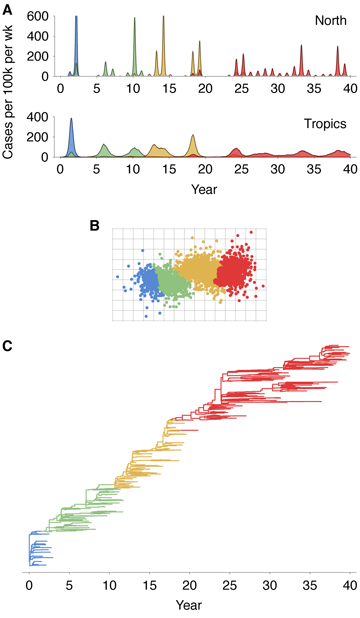
\includegraphics{figures/h1n1_mut}
	}
	\caption{\textbf{Simulation results showing epidemiological, antigenic and genealogical dynamics with weaker mutation}. (A) Weekly timeseries of incidence of viral infection in north and tropics regions. (B) Antigenic map depicting phenotypes of viruses sampled over the course of the simulation.  Grid lines show single units of antigenic distance. (C) Genealogical tree depicting the infection history of samples from the virus population.  Cluster assignments were used to color panels (A), (B) and (C) in a consistent fashion.  Here, $\mu = 5 \times 10^{-5}$, mean mutation size is 0.42 units and standard deviation of mutation size is 0.28 units.}
	\label{h1n1_mut}
\end{figure}
\vspace*{\fill}

\pagebreak

%%% Figure S9: h1n1_r0 %%%
\vspace*{\fill}
\begin{figure}[H]
	\centering
	\makebox[\textwidth]{
		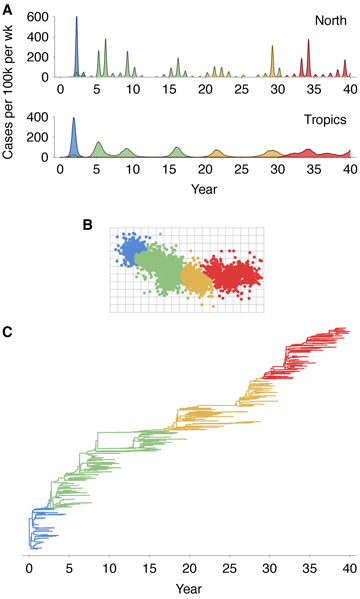
\includegraphics{figures/h1n1_r0}
	}
	\caption{\textbf{Simulation results showing epidemiological, antigenic and genealogical dynamics with lower intrinsic $R_0$}. (A) Weekly timeseries of incidence of viral infection in north and tropics regions. (B) Antigenic map depicting phenotypes of viruses sampled over the course of the simulation.  Grid lines show single units of antigenic distance. (C) Genealogical tree depicting the infection history of samples from the virus population.  Cluster assignments were used to color panels (A), (B) and (C) in a consistent fashion.  Here, $\beta = 0.3$, giving $R_0 = 1.5$.}
	\label{h1n1_r0}
\end{figure}
\vspace*{\fill}

\pagebreak

%%% Figure S10: 10dgrid %%%
\vspace*{\fill}
\begin{figure}[H]
	\centering
	\makebox[\textwidth]{	
		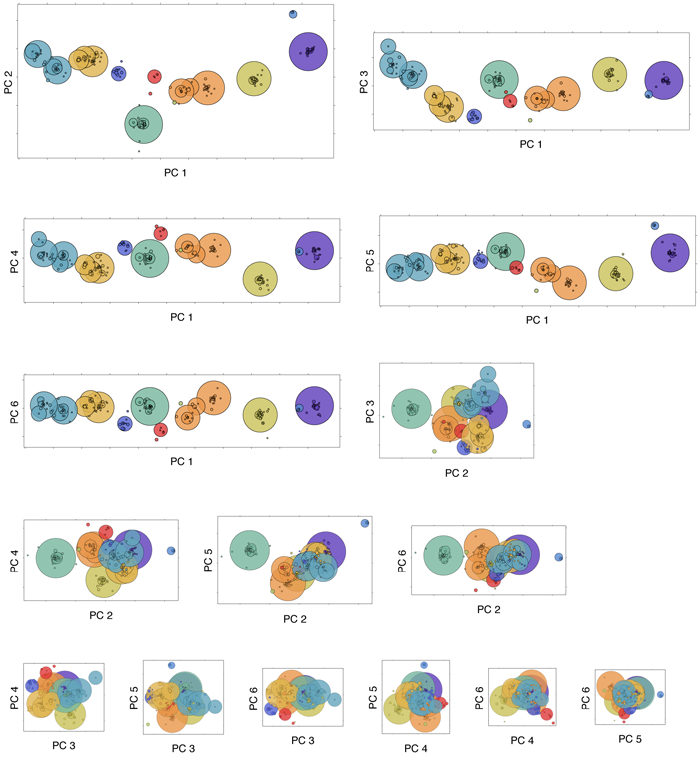
\includegraphics[width=0.9\textwidth]{figures/10dgrid}
	}
	\caption{\textbf{Principal components of antigenic variation under a 10-sphere mutation model}. Each panel shows 5991 samples of antigenic phenotype over the course of a 40-year simulation.  Each phenotype is represented as a bubble, with bubble area proportional to the number of samples with this phenotype.  Bubbles are colored based on clustering the 10-dimensional antigenic phenotypes.  The original 10-dimensional space was rotated using principal components analysis to give orthogonal axes in the order of their contribution to antigenic variation.  Each panel shows a two-dimensional slice of the this rotated space.  Principal components 7--10 were left out of the figure for clarity.}
	\label{10dgrid}
\end{figure}
\vspace*{\fill}



